\documentclass[10pt,a4paper, margin=1in]{article}
\usepackage{fullpage}
\usepackage{amsfonts, amsmath, pifont}
\usepackage{amsthm}
\usepackage{graphicx}

\usepackage{float}

\usepackage[utf8]{inputenc}
\usepackage{tkz-euclide}
\usepackage{tikz}
\usepackage{pgfplots}
\pgfplotsset{compat=1.13}

\usepackage{geometry}
 \geometry{
 a4paper,
 total={210mm,297mm},
 left=10mm,
 right=10mm,
 top=10mm,
 bottom=10mm,
 }
 % Write both of your names here. Fill exxxxxxx with your ceng mail address.
 \author{
  Aydın, Onur\\
  \texttt{e217126@metu.edu.tr}
  \and
  Bütün, Beyza\\
  \texttt{e2171411@ceng.metu.edu.tr}
}
\title{CENG 384 - Signals and Systems for Computer Engineers \\
Spring 2020 \\
Written Assignment 1}


\begin{filecontents}{q6.dat}
 n   xn
 1  1
 4   4
\end{filecontents}

\begin{filecontents}{q6-2.dat}
 n   xn
 3  -3
\end{filecontents}

\begin{filecontents}{q3.dat}
 n   xn
 -11 6
 -10 0
 -9  5
 -8  0
 -7  -4
 -6  0
 -5  0
 -4  3
 -3  0
 -2  -2
 -1  0
 0   1
 1   1  
 2   0
 3   0
 4   -4 
 5   5
 6   6
\end{filecontents}

\begin{document}
\maketitle

\noindent\rule{19cm}{1.2pt}

\begin{enumerate}

\item 
    \begin{enumerate}
    % Write your solutions in the following items.
    \item %write the solution of q1a
    Assume z = $x+yj$ and z+1 = j-3$\Bar{z}$ is given. 
    
    z+1 = $j-3 \Bar{z}$
    
    z+3$\Bar{z}$ = $j-1$
    
    $x+yj$+$3x-3yj$ = $j-1$
    
    $4x-2yj$ = $j-1$
    
    
    From this equation x=-1/4 and y=-1/2.
    \vspace{0.25cm}
    
    Therefore,
    
    z=$\frac{-1}{4}-\frac{1}{2}j$
    \vspace{0.5cm}
    
    $(i)$ ${\vert z \vert}^2$ = $(\sqrt{(-1/4)^2 + (-1/2)^2 })^2$ = 5/16
    \vspace{0.5cm}
    
    $(ii)$
    To plot z on complex plane, we should know the magnitude and the degree of it.
    
    As we calculated, the magnitude ${\vert z \vert}$ = $(\sqrt{(-1/4)^2 + (-1/2)^2 })$ = $\sqrt{5}/4$
    \vspace{0.25cm}
    
    Let's find the angle:
    
    $\angle z$ = $\theta$ = $\arctan(y/x)$
    
    $\arctan((-1/2)/(-1/4))$ + $\pi$  (We added $\pi$ because x,y$<$0)
    
    $\arctan(2) + \pi$ $\approx$ $243.43^{\circ}$
    
    \begin{figure}[h!]
    \centering
        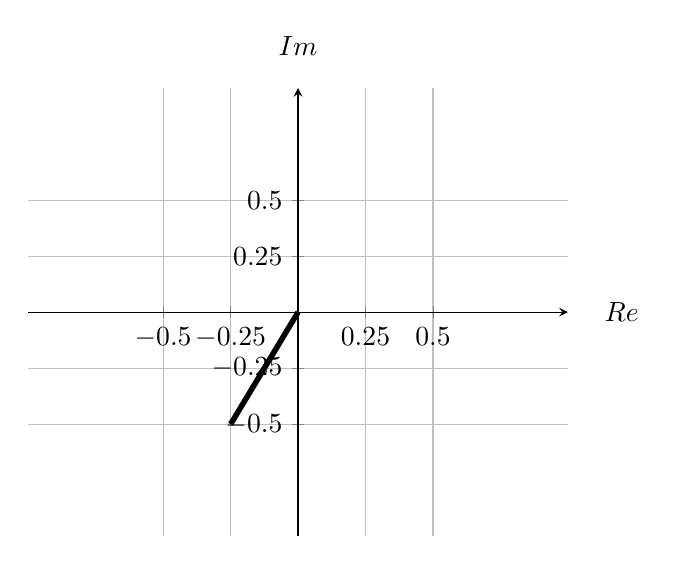
\begin{tikzpicture}[scale=1.0]
           \begin{axis}[
          axis lines=middle,
          xlabel={$Re$},
          ylabel={$Im$},
          xtick={ -0.5, -0.25, 0, 0.25, 0.5},
          ytick={-0.5 ,-0.25, 0, 0.25, 0.5},
          ymin=-1, ymax=1,
          xmin=-1, xmax=1,
          every axis x label/.style={at={(ticklabel* cs:1.05)}, anchor=west,},
          every axis y label/.style={at={(ticklabel* cs:1.05)}, anchor=south,},
          grid,
        ]
           \path[draw,line width=2pt] (-0.25,-0.5) -- (0,0);
           \end{axis}
        \end{tikzpicture}
        \caption{ z=$\frac{-1}{4}-\frac{1}{2}j$.}
        \label{fig:q1}
    \end{figure}
    
    
    \item %write the solution of q1b
    
    First, we know when $z$ = $re^{j\theta}$, $z^n$ = $(r e^{j\theta})^n$ = $r^n e^{jn\theta}$ and  $z^{1/n}$ = $r^{1/n} e^{j\theta/n}$
    
    $z^2$ = 25$j$ is given. So we can conclude that $z^2$ = 25$e^{(\pi/2)j}$.
    \vspace{0.25cm}
    
    Then, $z$ = $(25)^{1/2}e^{\frac{(\pi/2)j}{2}}$ = 5$e^{(\pi/4)j} = 5\cos{\frac{\pi}{4}}+j5\sin{\frac{\pi}{4}}$
    \vspace{0.25cm}
    
    \item %write the solution of q1c
    
    $1+j$ = $\sqrt{2}e^{(\pi/4)j}$
    
    $1-j$ = $\sqrt{2}e^{-(\pi/4)j}$
    
    $1-\sqrt{3}j$ = $2e^{-(\pi/3)j}$
    
    Then,
    \vspace{0.25cm}
    
    z = $\frac{(\sqrt{2}e^{(\pi/4)j})(2e^{-(\pi/3)j})}{\sqrt{2}e^{-(\pi/4)j}}$
    
    z = 2$e^{(\frac{\pi}{4}-\frac{\pi}{3}+\frac{\pi}{4})j}$
    
    z = 2$e^{(\pi/6)j}$ 
    \vspace{0.25cm}
    
    So, the magnitude ${\vert z \vert}$ = 2 and the angle is $\pi/6$.
    \vspace{0.25cm}
    
    \item %write the solution of q1d
    
    z = $je^{-j\pi/2}$ = $e^{j\pi/2} e^{-j\pi/2}$ = $e^{0j}$ = 1
    
    \end{enumerate}


\item %write the solution of q2
The signal can be represented as
$
x(t)
\begin{cases} 
      0 & 0 \leq t \leq 1 \\
      t-1 & 1 < t \leq 3 \\
      2 & 3 < t \leq 5 \\
      7-t & 5 < t \leq 7 \\
      0 & 7 < t \leq 8 \\
   \end{cases}
$
\vspace{0.25cm}

To find x(2t-2), all t should be 2t-2. Therefore,
\vspace{0.25cm}

$
x(2t-2)
\begin{cases} 
      0 & 0 \leq 2t-2 \leq 1 \\
      2t-3 & 1 < 2t-2 \leq 3 \\
      2 & 3 < 2t-2 \leq 5 \\
      9-2t & 5 < 2t-2 \leq 7 \\
      0 & 7 < 2t-2 \leq 8 \\
   \end{cases}
$
==
$
x(2t-2)
\begin{cases} 
      0 & 1 \leq t \leq 3/2 \\
      2t-3 & 3/2 < t \leq 5/2 \\
      2 & 5/2 < t \leq 7/2 \\
      9-2t & 7/2 < t \leq 9/2 \\
      0 & 9/2 < t \leq 5 \\
   \end{cases}
$
\vspace{0.25cm}

Finally;

$
y(t) = \frac{1}{2}x(2t-2)
\begin{cases} 
      0 & 1 \leq t \leq 3/2 \\
      t-3/2 & 3/2 < t \leq 5/2 \\
      1 & 5/2 < t \leq 7/2 \\
      9/2-t & 7/2 < t \leq 9/2 \\
      0 & 9/2 < t \leq 5 \\
   \end{cases}
$
\vspace{0.25cm}

And $y(t) = \frac{1}{2}x(2t-2)$ plot will be as the following.

\begin{figure}[h!]
    \centering
        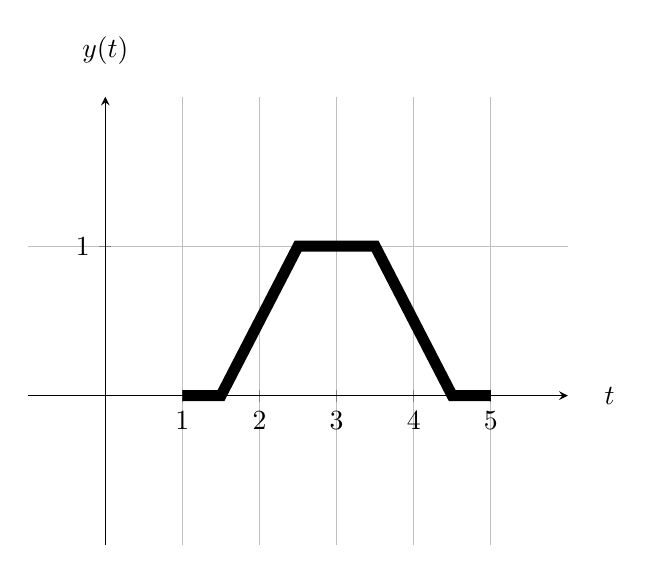
\begin{tikzpicture}[scale=1.0]
           \begin{axis}[
          axis lines=middle,
          xlabel={$t$},
          ylabel={$y(t)$},
          xtick={0, 1, 2, 3, ..., 5},
          ytick={0, 1},
          ymin=-1, ymax=2,
          xmin=-1, xmax=6,
          every axis x label/.style={at={(ticklabel* cs:1.05)}, anchor=west,},
          every axis y label/.style={at={(ticklabel* cs:1.05)}, anchor=south,},
          grid,
        ]
           \path[draw,line width=4pt] (1,0) -- (3/2,0) -- (5/2,1) -- (7/2,1) -- (9/2,0) -- (5,0);
           \end{axis}
        \end{tikzpicture}
        \caption{$t$ vs. $ y(t) $.}
        \label{fig:q2}
    \end{figure}

\clearpage
\item      
    
    \begin{enumerate}
    \item %write the solution of q3a
    
    $x[-n] + x[2n-1]$ can be drawn as the following:
    
    \begin{figure}[h!]
    \centering
    \begin{tikzpicture}[scale=1.5] 
      \begin{axis}[
          axis lines=middle,
          xlabel={$n$},
          ylabel={$\boldsymbol{x[-n] + x[2n-1] }$},
          xtick={ -12, -11, -10, -9, -8, -7, -6, -5, -4, -3, -2 ,-1, 0 ,  ..., 7},
          ytick={-4, -3, -2, -1, ..., 6},
          ymin=-4, ymax=6,
          xmin=-11, xmax=7,
          every axis x label/.style={at={(ticklabel* cs:1.05)}, anchor=west,},
          every axis y label/.style={at={(ticklabel* cs:1.05)}, anchor=south,},
          grid,
        ]
        \addplot [ycomb, black, thick, mark=*] table [x={n}, y={xn}] {q3.dat};
      \end{axis}
    \end{tikzpicture}
    \caption{$n$ vs. $x[-n] + x[2n-1]$.}
    \label{fig:q3}
\end{figure}
\vspace{0.25cm}   

    \item %write the solution of q3b
    
    $x[-n] + x[2n-1]$  = $6\delta[n+11] + 5\delta[n+9] - 4\delta[n+7] + 3\delta[n+4] - 2\delta[n+2] + \delta[n] + \delta[n-1] - 4\delta[n-4] + 5\delta[n-5] + 6\delta[n-6]  $
    
    \end{enumerate}
\vspace{0.25cm}

\item 
    \begin{enumerate}
    \item %write the solution of q4a
    
    $x[n]$ = $7sin[\frac{5\pi}{8}n -\frac{2\pi}{3}] + 2cos[\frac{2\pi}{3}n]$
    \vspace{0.25cm}
    
    For only $sin[\frac{5\pi}{8}n -\frac{2\pi}{3}]$ part,
    
    $N_1 = \frac{2\pi}{\frac{5\pi}{8}}k = \frac{16}{5}k$ If we choose k=5, $N_0=16$
    \vspace{0.25cm}
    
    For only $cos[\frac{2\pi}{3}n]$ part, 
    
    $N_2 = \frac{2\pi}{\frac{2\pi}{3}}k = 3k$ If we choose k=1, $N_0=3$ 
    \vspace{0.25cm}
    
    The signal $x[n]$ is periodic with fundamental period $N_0=$LCM$(16,3)=48$.
    \vspace{0.25cm}
    
    \item %write the solution of q4b
    
    $x[n]$ = $3cos[5n -\frac{3\pi}{4}]$
    \vspace{0.25cm}
    
    The signal $x[n]$ is not periodic because
    
    $N = \frac{2\pi}{5}k$, where there is no integer $k$ to make the fundamental period the smallest possible integer.
    \vspace{0.25cm}
    
    \item %write the solution of q4c
    
    $x(t)$ = $4sin(5 \pi t -\frac{3\pi}{5})$ 
    \vspace{0.25cm}
    
    $T = \frac{2\pi}{5\pi}k = \frac{2}{5}k$ 
    
    
    The signal $x(t)$ is periodic where $T=\frac{2}{5}k$, if we choose k=1, $T_0=\frac{2}{5}$. 
    
    \item %write the solution of q4d
    
    $x(t)=x(t+T_0)=je^{j2t}=je^{j2(t+T_0)}$
    \vspace{0.25cm}
    
    $e^{j2T_0}=1=cos(2T_0) + jsin(2T_0)$
    
    $2T_0=2\pi k$
    
    The signal x(t) is periodic. If we choose k as 1, the fundamental period $T_0=\pi$.
    \vspace{0.25cm}
    
    \end{enumerate}

\item %write the solution of q5

The signal is neither even nor odd, so we can find the even
and odd compositions of the signal as the following:
\vspace{0.25cm}

x(t) = Odd$\{$x(t)$\}$ + Ev$\{$x(t)$\}$ 


Odd$\{$x(t)$\}$ = 1/2(x(t)-x(-t)) 

Ev$\{$x(t)$\}$ = 1/2(x(t)+x(-t)) 
\vspace{0.25cm}

The figures of the odd and even signals are as follows:

\begin{figure}[h!]
    \centering
        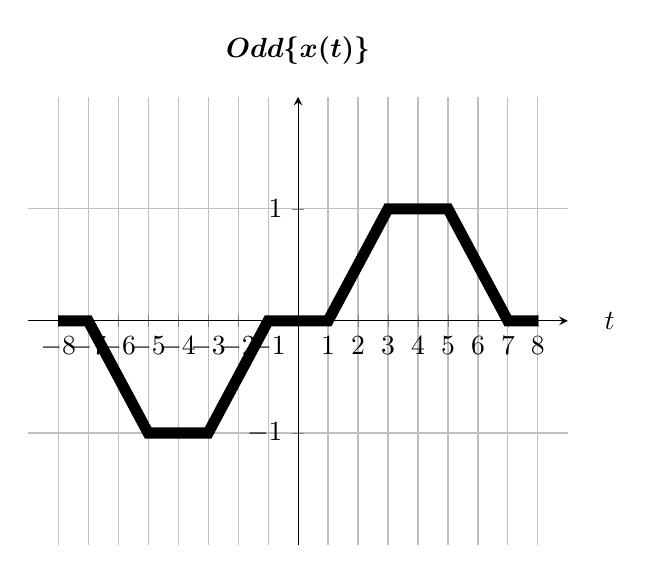
\begin{tikzpicture}[scale=1.0]
           \begin{axis}[
          axis lines=middle,
          xlabel={$t$},
          ylabel={$\boldsymbol{Odd\{x(t)\}}$},
          xtick={-8, -7, ..., -3, -2, -1, 0, 1, 2, 3, ..., 8},
          ytick={-1, 0, 1},
          ymin=-2, ymax=2,
          xmin=-9, xmax=9,
          every axis x label/.style={at={(ticklabel* cs:1.05)}, anchor=west,},
          every axis y label/.style={at={(ticklabel* cs:1.05)}, anchor=south,},
          grid,
        ]
           \path[draw,line width=4pt] (-8,0) -- (-7,0) -- (-5,-1) -- (-3,-1) -- (-1,0) -- (0,0) -- (1,0) -- (3,1) -- (5,1) -- (7,0) -- (8,0);
           \end{axis}
        \end{tikzpicture}
        \caption{$t$ vs. $ Odd\{x(t)\} $.}
        \label{fig:q2}
    \end{figure}
    
 
 
\begin{figure}[h!]
    \centering
        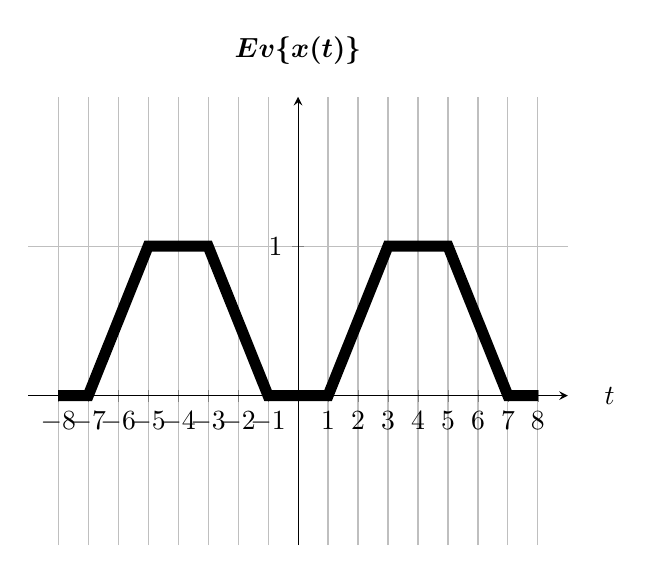
\begin{tikzpicture}[scale=1.0]
           \begin{axis}[
          axis lines=middle,
          xlabel={$t$},
          ylabel={$\boldsymbol{Ev\{x(t)\}}$},
          xtick={-8, -7, ..., -3, -2, -1, 0, 1, 2, 3, ..., 8},
          ytick={0, 1},
          ymin=-1, ymax=2,
          xmin=-9, xmax=9,
          every axis x label/.style={at={(ticklabel* cs:1.05)}, anchor=west,},
          every axis y label/.style={at={(ticklabel* cs:1.05)}, anchor=south,},
          grid,
        ]
           \path[draw,line width=4pt] (-8,0) -- (-7,0) -- (-5,1) -- (-3,1) -- (-1,0) -- (0,0) -- (1,0) -- (3,1) -- (5,1) -- (7,0) -- (8,0);
           \end{axis}
        \end{tikzpicture}
        \caption{$t$ vs. $ Ev\{x(t)\}$.}
        \label{fig:q2}
    \end{figure}
     
\vspace{0.5cm}
\item 
    \begin{enumerate}
    \item %write the solution of q6a
    
    x(t) = u(t-1) - 3u(t-3) + 4u(t-4)
    \vspace{0.25cm}
    
    \item %write the solution of q6b
    
    We know that the unit step function u(t) = $ \int_{-\infty}^{t} \delta(\tau)d\tau  $ and $\delta(t) = \frac{du(t)}{dt}$. 
    \vspace{0.25cm}
    
    Therefore;
    
    $\frac{dx(t)}{dt}$ = $\delta(t-1) - 3\delta(t-3) +4\delta(t-4)$
    \vspace{0.25cm}
    
    The following figure shows the unit impulse function:
    
    
    
    \begin{figure}[h!]
    \centering
    \begin{tikzpicture}[scale=1.0] 
      \begin{axis}[
          axis lines=middle,
          xlabel={$t$},
          ylabel={$\boldsymbol{\delta(t)}$},
          xtick={ 0, 1, 2, 3, 4},
          ytick={-3, -2, -1, 0, 1, 2, 3, 4},
          ymin=-4, ymax=4,
          xmin=-1, xmax=5,
          every axis x label/.style={at={(ticklabel* cs:1.05)}, anchor=west,},
          every axis y label/.style={at={(ticklabel* cs:1.05)}, anchor=south,},
          grid,
        ]
        \addplot [ycomb, black, thick, mark=triangle, mark options={rotate=180}] table [x={n}, y={xn}] {q6-2.dat};
        \addplot [ycomb, black, thick, mark=triangle] table [x={n}, y={xn}] {q6.dat};
      \end{axis}
    \end{tikzpicture}
    \caption{$t$ vs. $\delta(t)$.}
    \label{fig:q6}
\end{figure}
    
    \end{enumerate}

\end{enumerate}
\end{document}

